\documentclass[12p]{article}
\usepackage{tikz}
\usepackage{graphicx}
\usepackage[export]{adjustbox}

\begin{document}
\begin{center}
Rolf-Benz-Schule Nagold\\
Physik-Labor\\
Lehrer: Herr Schlinger \\
\vspace{20pt}
\huge Freier Fall vs. Waagerechter Wurf\\
\vspace{80pt}
\large 
Amar Uka\\
Daniel Renschler\\
Melih Bektas\\
Lukas Naumann\\
\vspace{18pt}
Fälligkeitsdatum: 9. Dezember 2022 \\
Abgegeben: 04. Dezember 2022 \\
\vspace{18pt}
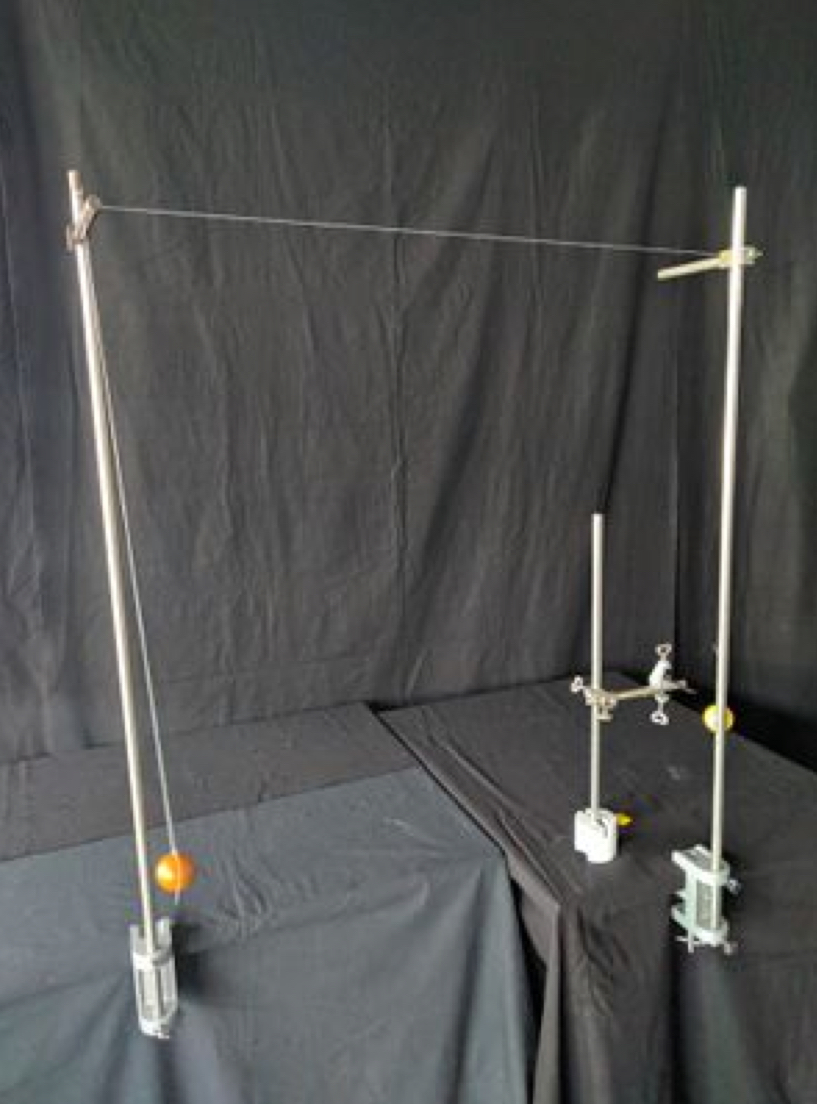
\includegraphics[scale=0.23]{versuch freier fall.jpeg}
\end{center}
\pagenumbering{gobble}

\clearpage

\section*{Ziel des Versuchs}
Experimentelle Bestimmung der Falldauer beim waagerechten Wurf, im Vergleich zum
Senkrechten Fall.

\section*{Thematischer Kontext und ggf. die zu überprüfende Behauptung.}
Ein Fall kann entweder "normal" senkrecht stattfinden oder mit einer
Beeinflussung, z.B. in x-Richtung, wie im folgenden Versuch. Ziel war
herauszufinden ob die Gewichte gleichzeitig zu Boden fallen, Gewicht 1
senkrecht, und Gewicht 2 mit einer Geschwindigkeitskomponente in x.Richtung
durch einen vorherigen Pendelschwung.

\section*{Ort und Zeit der Durchführung, Namen der Experimentatoren}
Der Versuch wurde in der Rolf-Benz-Schule Nagold, Raum 349, am 25. November 2022
durchgeführt, von Amar Uka, Daniel Renschler, Melih Bektas und Lukas Naumann.

\section*{Beschreibung und ggf. Abbildung des Versuchsaufbaus}
Zwei Gewichte wurden an einer Schnur festgemacht, welche über Stativstangen
gespannt wurde, die eine Kugel wird Aus einer höhe gefallen lassen auf eine
Rasierklinge, die am untersten Punkt des "Pendelgewichts" steht.
\begin{figure}[!h]
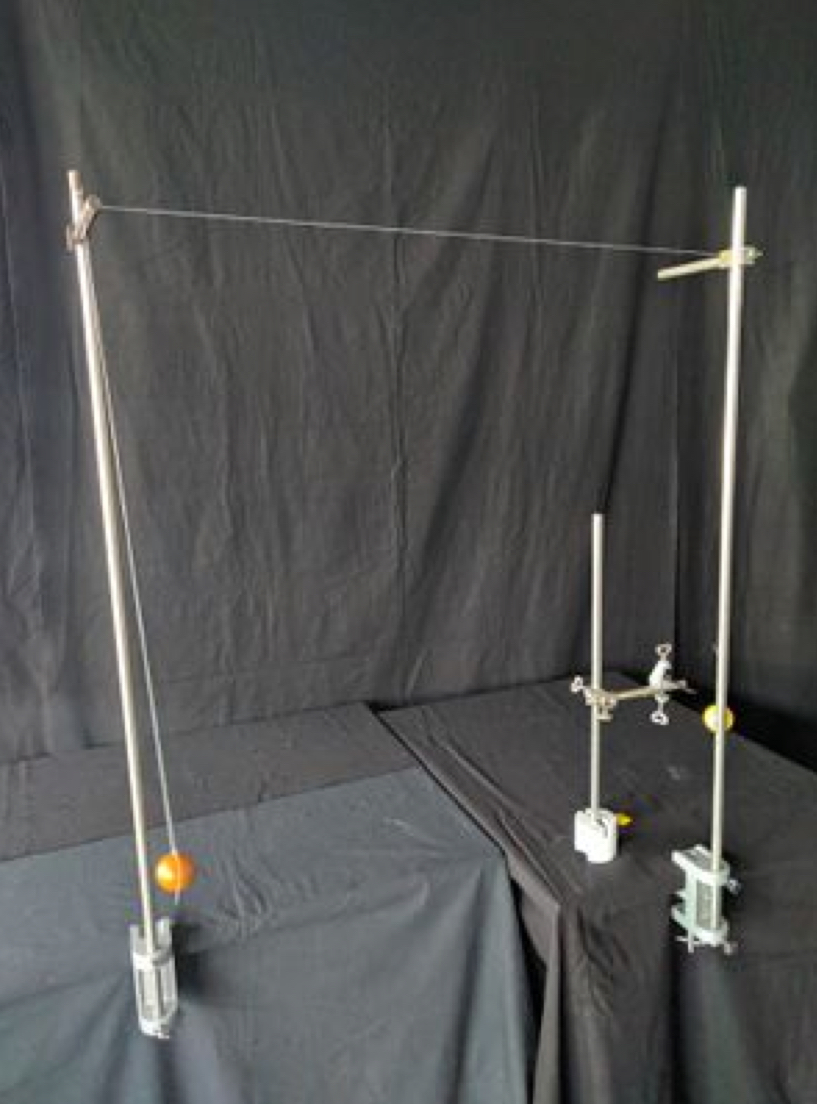
\includegraphics[scale=0.1]{versuch freier fall.jpeg}
\end{figure}

\section*{Beschreibung der Versuchsdurchführung}
Die zwei Gewichte werden in einen Fall oder Wurf  versetzt indem die "Pendel-Kugel" an
ihrer Pendelschnur am tiefsten Punkt durchschnitten wird und mit maximalem
Schwung Waagerecht geworfen wird. Die Andere Kugel fängt an zu fallen sobald die
gemeinsame Schnur getrennt wird, sodass die Gewichte zur exakt gleichen Zeit in
ihre Bewegung kommen.


\section*{Messergebnisse und ggf. Veranschaulichung}
\begin{center}
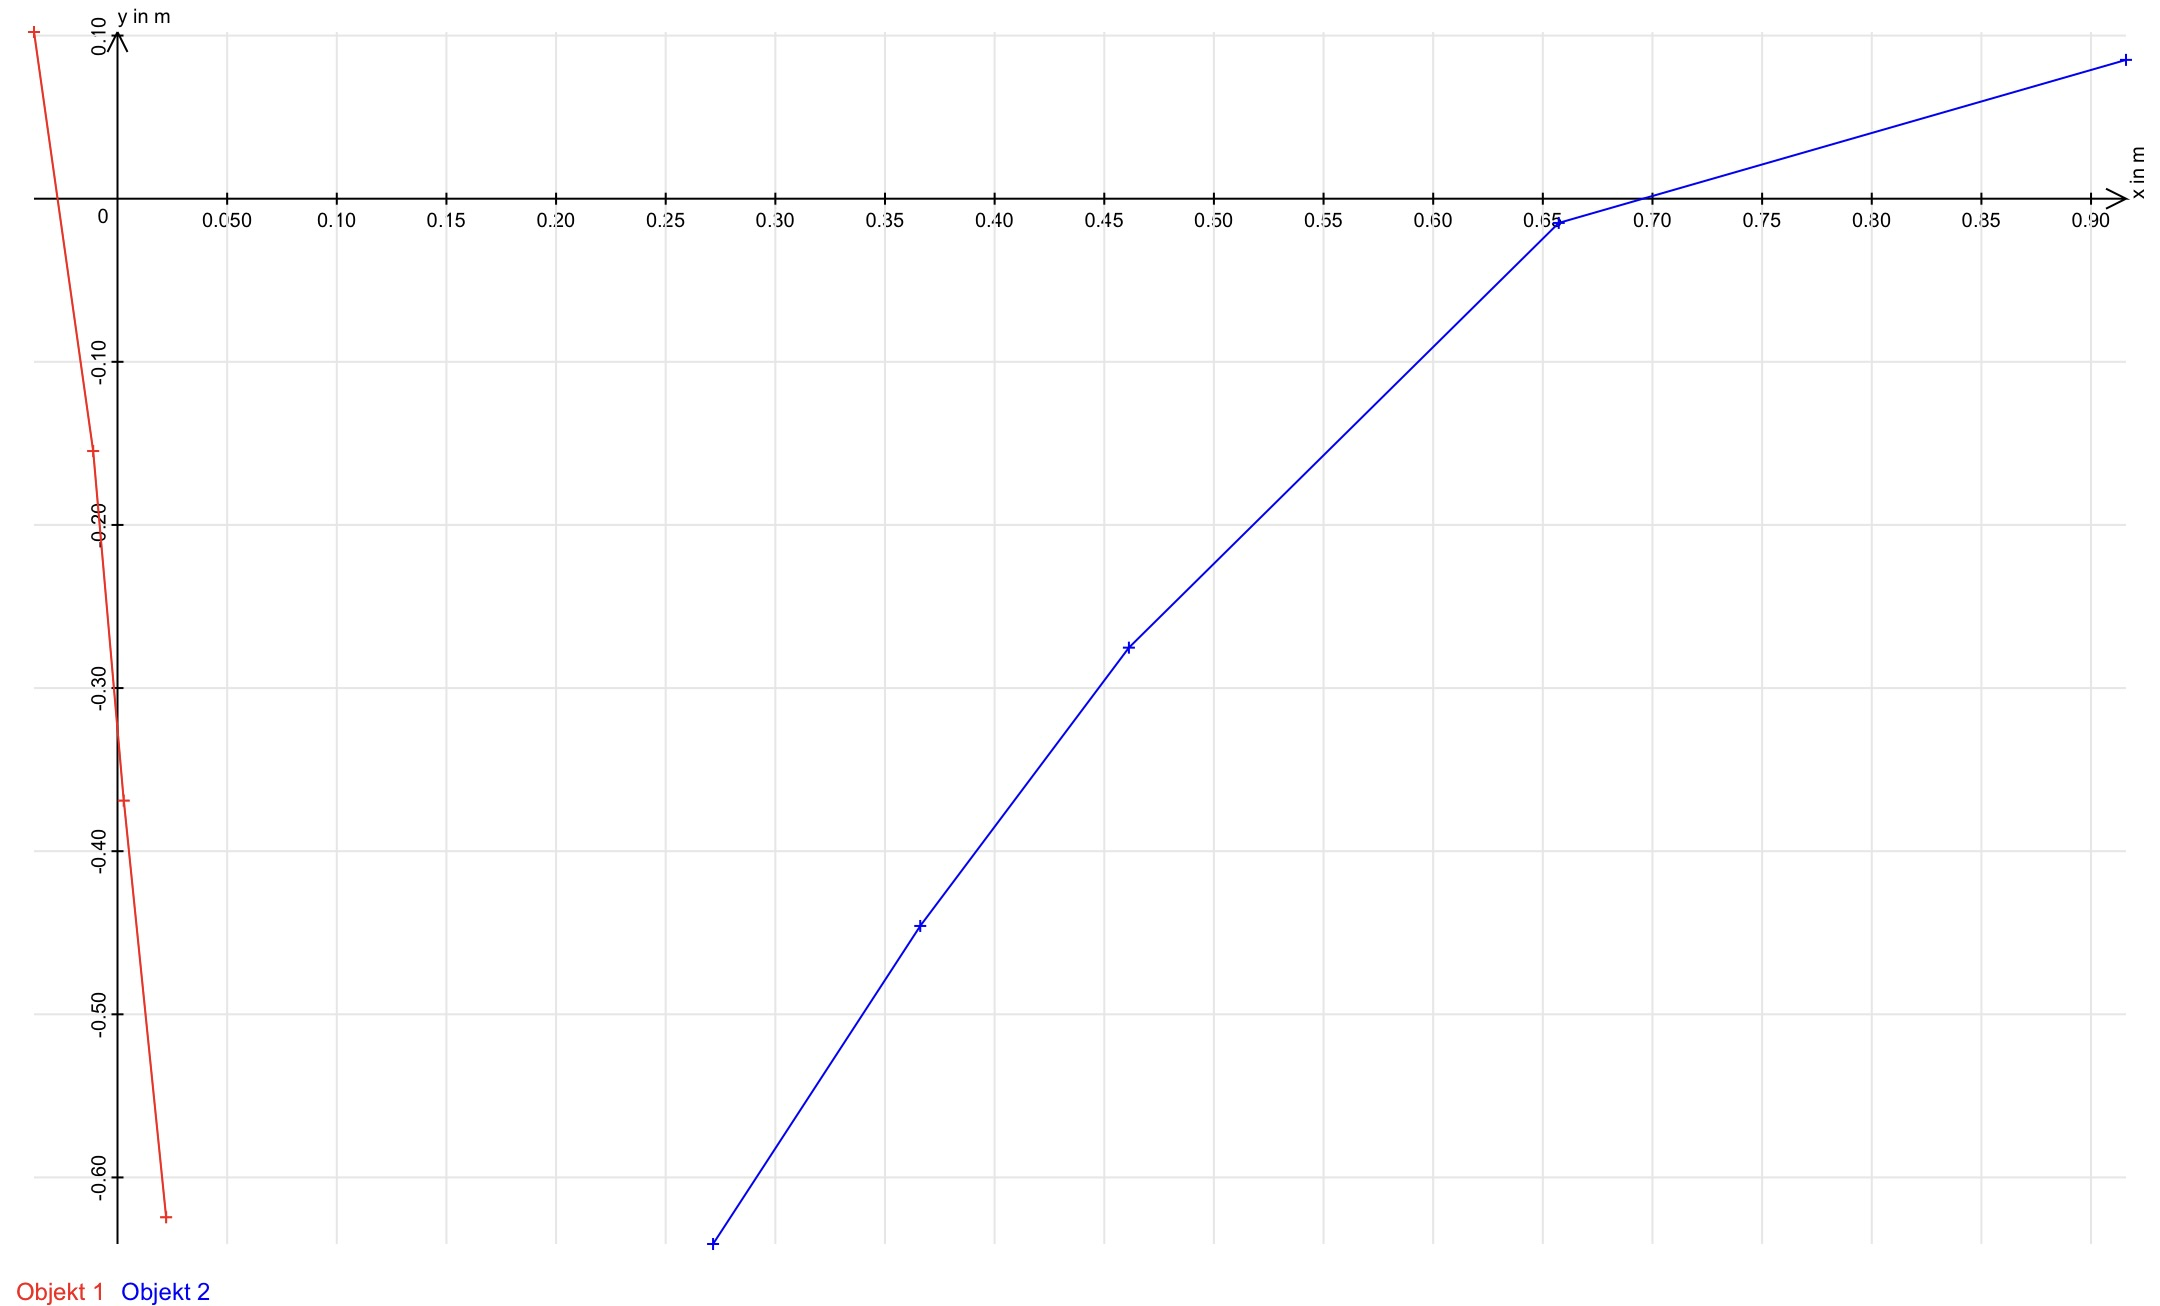
\includegraphics[width=\textwidth]{messergebnisse.jpeg}
\end{center}

\section*{Fehlerbetrachtung}
Die Fehlerbetrachtung kann hier nur in einem sehr groben Rahmen durchgeführt
werden da die Messergebnisse sowie der Versuch nicht von unserer Gruppe
durchgeführt wurden, wir hatten erst Probleme mit Viana und später mit dem iPad
selbst als der Akku leer ging. Im folgenden sind die Fehler, die wir von der
durchführenden Gruppe mitgeteilt bekommen habe.
Es wurde nicht im richtigen Moment losgelassen, die Messung von Viana war nicht
genau, die Gewichte waren nicht auf der gleichen Höhe und die Stäbe der Schnur
(Halterung) waren auch nicht auf gleicher Höhe.

\section*{Interpretation und Schlussfolgerung}
Wenn man die Reibung mit der Luft insignifikant erklärt auf der kurzen Distanz
kann man sagen die Gewichte sind gleich schnell zu Boden gefallen/geworfen
worden, senkrecht sowie Waagerecht. Zumindest solang sie auf gleicher Höhe
starten und gleichzeitig mit ihrer Bewegung versetzt werde.


\end{document}
